\chapter{Dise�o de las partes mec�nicas TODO}

La mayor parte de las piezas que monta Raider han sido redise�adas para mejorar su funci�n y/o permitir el alojamiento de nuevos dispositivos. Adem�s, al haber sido dise�adas con OpenSCAD, ha sido posible parametrizarlas para facilitar modificaciones futuras. Acciones como agregar a una pieza un soporte para un sensor determinado son ahora mucho mas r�pidas.

\section{Cabeza}

Uno de los principales objetivos del proyecto, el tomar datos del entorno con una c�mara, requiere  el dise�o y montaje se un soporte m�vil en el que poder albergar la webcam. Se ha decidido colocar la webcam en la cabeza del robot por ser la zona mas alta del robot y por tener espacio para su libre movimiento. La cabeza estar� formada por cuatro piezas: Bancada del servo, ch�sis, tapa con ranura para el cable y soporte de la c�mara. En la imagen de la figura \ref{piezascabeza} se muestran las piezas.

\begin{figure}[h]
\centering
\begin{tabular}{ >{\centering\arraybackslash}m{0.5\textwidth} >{\arraybackslash}m{0.5\textwidth}}
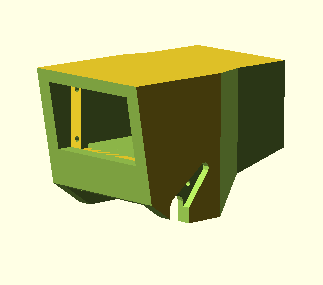
\includegraphics[width=0.4\textwidth]{figuras/cabeza} & 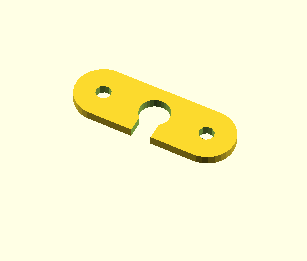
\includegraphics[width=0.4\textwidth]{figuras/tapacabeza}  \\
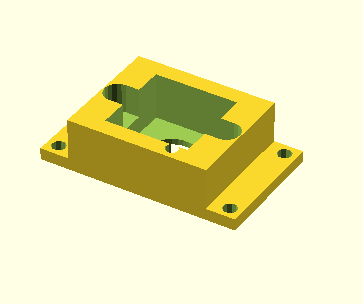
\includegraphics[width=0.4\textwidth]{figuras/chasislifecam} & 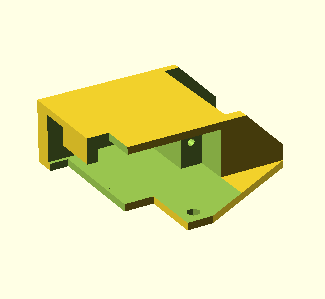
\includegraphics[width=0.4\textwidth]{figuras/cuello}  \\
\end{tabular}
\caption{Piezas necesarias para montar la cabeza}
\label{piezascabeza}
\end{figure} 
\FloatBarrier

\section{Cintura}

Como se coment� en el apartado TODO , ha sido necesario incluir un servo adicional en la cintura que permita realizar movimientos horizontales del tronco del robot respecto a la piernas. Como puede verse en la figura \ref{piezascintura}, consta de dos piezas que aprisionan el servomotor y otra mas que se utilizar� como soporte de la bater�a.

\begin{figure}[h]
\centering
\begin{tabular}{ >{\centering\arraybackslash}m{0.5\textwidth} >{\arraybackslash}m{0.5\textwidth}}
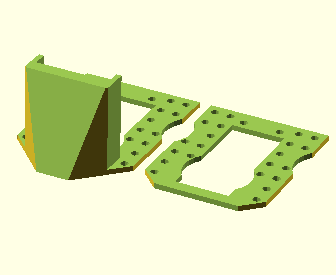
\includegraphics[width=0.4\textwidth]{figuras/cintura} & 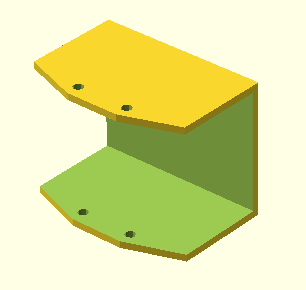
\includegraphics[width=0.4\textwidth]{figuras/soportebat}  \\
\end{tabular}
\caption{Piezas necesarias para montar la cintura}
\label{piezascintura}
\end{figure} 
\FloatBarrier 

\section{Tronco}

Para dise�ar el tronco exiten varias premisas. Necesitamos un cuerpo que permita albergar el nuevo controlador, soportar los servos de los hombros, tener una zona adecuada para montar la cabeza y una base firme que permita atornillarlo al nuevo servo de la cintura. El la imagen de la figura \ref{piezastronco} se muestran las piezas necesarias para montar el tronco: Pecho, espalda y protector.

\begin{figure}[h]
\centering
\begin{tabular}{ >{\centering\arraybackslash}m{0.5\textwidth} >{\arraybackslash}m{0.5\textwidth}}
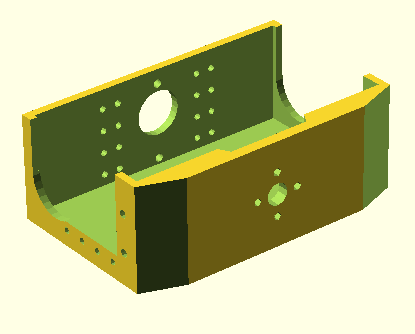
\includegraphics[width=0.4\textwidth]{figuras/pecho} & 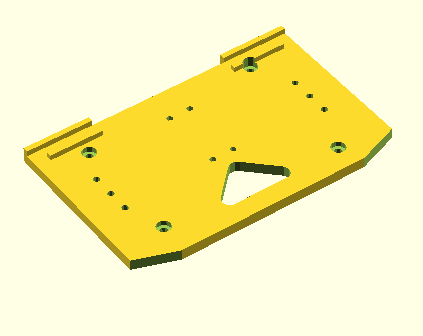
\includegraphics[width=0.4\textwidth]{figuras/espalda}  \\
\end{tabular}
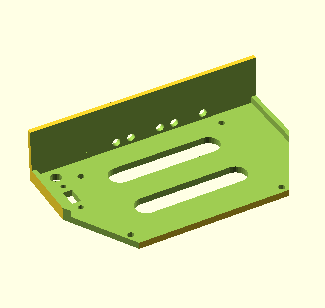
\includegraphics[width=0.4\textwidth]{figuras/protector} \\
\caption{Piezas necesarias para montar el tronco}
\label{piezastronco}
\end{figure} 
\FloatBarrier

\section{Brazos}

En este apartado se han dise�ado diferentes tramos tramos del brazo. Con ello se ha dotarle de una total modularidad, separando uniones entre servos, soportes para sensores y protectores. Gracias a esto, es muy sencillo sustituir unas piezas por otras. En este caso se han inclu�do sensores infrarrojos en los antebrazos, sin embargo, si se necesitase cambiarlos por sensores de ultrasonidos (o cualquier otro sensor) solo ser�a necesario modificar y reimprimir la bancada del sensor. En la figura \ref{piezasbrazo}

\begin{figure}[h]
\centering
\begin{tabular}{ >{\centering\arraybackslash}m{0.5\textwidth} >{\arraybackslash}m{0.5\textwidth}}
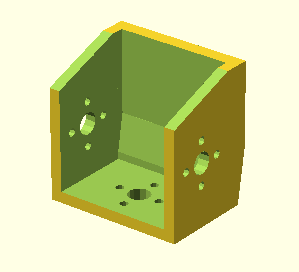
\includegraphics[width=0.4\textwidth]{figuras/hombro} & 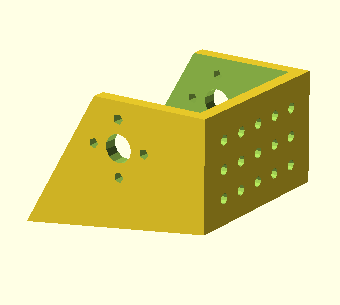
\includegraphics[width=0.4\textwidth]{figuras/codo}  \\
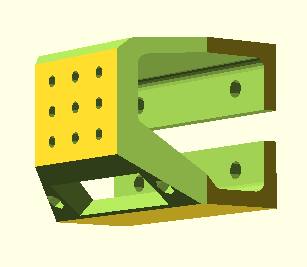
\includegraphics[width=0.4\textwidth]{figuras/antebrazo} & 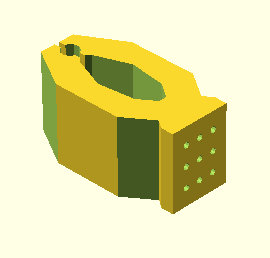
\includegraphics[width=0.4\textwidth]{figuras/gripper}  \\
\end{tabular}
\caption{Piezas necesarias para montar un brazo}
\label{piezasbrazo}
\end{figure} 
\FloatBarrier

\section{Piernas}

En cuanto a las piernas, mostradas en la figura \ref{piezaspierna}, se han modificado con dos objetivos: Rigidificar sus tramos y acortar levemente su longitud para descargar peso en las articulaciones. Al mismo tiempo, ayudar�n a bajar el centro de gravedad del robot y aumentar su estabilidad.

\begin{figure}[h]
\centering
\begin{tabular}{ >{\centering\arraybackslash}m{0.5\textwidth} >{\arraybackslash}m{0.5\textwidth}}
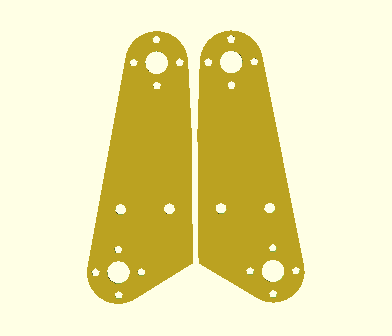
\includegraphics[width=0.4\textwidth]{figuras/pierna1} & 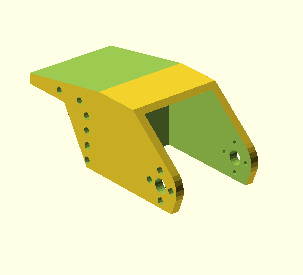
\includegraphics[width=0.4\textwidth]{figuras/pierna2}  \\
\end{tabular}
\caption{Piezas necesarias para montar una pierna}
\label{piezaspierna}
\end{figure} 
\FloatBarrier

\section{Pies y tobillos}

El dise�o de los pies se ha planteado de forma que cumpla las especificaciones del reglamento del campeonato CEABOT y al mismo tiempo tenga la mayor superficie posible. A priori, parece sencillo suponer que cuanto mayor sea la extensi�n del pie mayor ser� la estabilidad del robot, sin embargo, tambi�n es muy importante controlar como se distribuye el peso en la planta. Con el objetivo de concentrar el peso en el centro de la planta, se ha realizado un redise�o completo del tobillo, tal y como puede observarse en las piezas de la figura \ref{piezaspie}

\begin{figure}[h]
\centering
\begin{tabular}{ >{\centering\arraybackslash}m{0.5\textwidth} >{\arraybackslash}m{0.5\textwidth}}
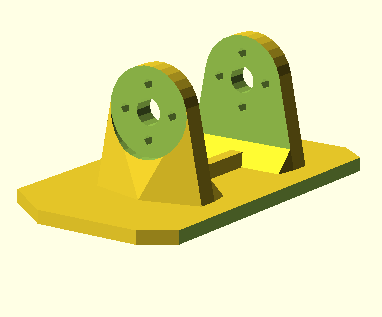
\includegraphics[width=0.4\textwidth]{figuras/pie} & 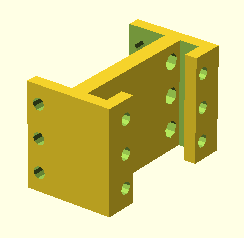
\includegraphics[width=0.4\textwidth]{figuras/tobillo}  \\
\end{tabular}
\caption{Piezas necesarias para montar un pie}
\label{piezaspie}
\end{figure}
\FloatBarrier
